\documentclass[12pt]{article}

\usepackage[T1]{fontenc}
\usepackage[utf8]{inputenc}
\usepackage[brazil]{babel}
\usepackage{mathptmx}
\usepackage[a4paper,left=3.1cm,right=3.1cm,top=3.0cm,bottom=3.0cm]{geometry}
\usepackage{graphicx}
\usepackage{booktabs}
\usepackage{amsmath,amssymb}
\usepackage{url}
\usepackage[hidelinks]{hyperref}
\usepackage{xurl}
\setlength{\emergencystretch}{2em}
\usepackage[labelfont=bf,font=small,labelsep=period]{caption}
\usepackage{enumitem}
\usepackage{times}

\setlength{\parindent}{1.2em}
\setlength{\parskip}{0.25em}
\renewcommand{\baselinestretch}{1.05}

\makeatletter
\renewenvironment{thebibliography}[1]{%
  \section*{Refer\^encias}%
  \list{}{\usecounter{enumiv}\let\p@enumiv\@empty%
    \renewcommand\theenumiv{\@arabic\c@enumiv}%
    \setlength{\labelwidth}{0pt}\setlength{\labelsep}{0pt}%
    \setlength{\leftmargin}{1.6em}\setlength{\itemindent}{-1.6em}%
    \setlength{\itemsep}{0.35em}\setlength{\parsep}{0pt}}%
  \small\sloppy\clubpenalty4000\widowpenalty4000%
  \let\@noitemerr\relax}%
 {\endlist}
\makeatother

\newenvironment{sbcabstract}[1]
  {\begin{list}{}{\setlength{\leftmargin}{1.2em}\setlength{\rightmargin}{1.2em}}%
   \item[]\itshape\textbf{\upshape\textit{#1}}\hspace{0.4em}}
  {\end{list}}

\begin{document}

\begin{center}
{\large\bfseries APRENDIZADO DE MÁQUINA SOBRE OBSERVÁVEIS PÚBLICOS DE QKD:\\[0.2em]
CLASSIFICAÇÃO DE ATAQUES, OTIMIZAÇÃO DA TAXA DE CHAVE\\[0.2em]
E SINCRONISMO EM ENLACES COM \emph{DECOY STATES}}

\vspace{1.0em}
{\bfseries Alexandre O. S. Santos\textsuperscript{1,2}}

\vspace{0.9em}
\textsuperscript{1}Quantum Industrial Innovation - QuIIN\\
Senai CIMATEC -- Salvador, BA -- Brazil

\vspace{0.5em}
\textsuperscript{2}Latin America Quantum Computing Center - LAQCC\\
Senai CIMATEC -- Salvador, BA -- Brazil

\vspace{0.7em}
{\ttfamily\small alexandreoliversan1@gmail.com, alexandre.ssantos@fbter.org.br}
\end{center}

\vspace{0.8em}

\begin{sbcabstract}{Abstract.}
A deployed decoy-state QKD link monitors itself with a single statistic: the
quantum bit error rate (QBER). That test is sound and operationally weak. It
fires late, it fires for the weather, and it is blind to every attack that does
not disturb the error rate. This work develops a classical machine-learning
layer that consumes only the observables the two ends already publish --- gains
and error rates per intensity, the vacuum count, the decoy bounds --- plus a
cable thermometer. Attacks are modelled as modifications of the per-photon-number
yields, so that what Bob observes is derived rather than asserted, and an attack
with no physical signature acquires none in the dataset. On 90{,}720 settling
periods of simulated sessions, a QBER threshold calibrated to a 1\% false-alarm
budget detects one of four attacks; a gradient-boosting classifier over the same
public record reaches a macro F1 of 0.830 and separates eavesdropping from
thermal drift. Two further controllers share the same physics: an
advantage-actor-critic agent that tunes the transmitter intensities and clock,
raising the provable secret key rate by 8.8\% to 18.9\% over a commissioning
baseline across 25--80~km, and a timing predictor that keeps the detector gate
aligned against the thermal drift of the propagation delay. The evaluation is
deliberately adverse: attacks ramp in, work in bursts, and 40\% of them run
during a simultaneous thermal excursion. The central operational finding is that
precision under a realistic prior is governed by the decision rate, not by the
model --- at a one-second settling period the best detector yields 0.22
precision, and at five seconds, with a calibrated decision threshold, it reaches
1.00 at the cost of detection delay. Against 575 days of a deployed link of the
Cambridge Quantum Network, a QBER threshold calibrated at commissioning to a 1\%
budget fires on 16.5\% of benign days, the measured cost of one point of QBER
agrees with the model's key-rate physics to within 6\%, and the coexistence
penalty has the predicted Raman form.
\end{sbcabstract}

\vspace{0.4em}
\noindent\textbf{\textit{Keywords}}: \textit{Quantum Key Distribution, Decoy States,
Attack Detection, Reinforcement Learning, Secret Key Rate, Time Synchronisation,
Field Validation.}

\vspace{0.9em}

\begin{sbcabstract}{Resumo.}
Um enlace de QKD com \emph{decoy states} implantado monitora a si mesmo por uma
única estatística: a taxa de erro quântica (QBER). O teste é correto e
operacionalmente fraco --- dispara tarde, dispara por causa do clima e é cego a
todo ataque que não perturba a taxa de erro. Este trabalho desenvolve uma camada
clássica de aprendizado de máquina que consome apenas os observáveis que as duas
pontas já publicam --- ganhos e taxas de erro por intensidade, contagem de vácuo
e as cotas de \emph{decoy} --- somados a um termômetro no cabo. Os ataques são
modelados como modificações dos \emph{yields} por número de fótons, de modo que o
que Bob observa é derivado e não postulado, e um ataque sem assinatura física não
ganha assinatura no conjunto de dados. Em 90.720 períodos de acerto de sessões
simuladas, um limiar de QBER calibrado para 1\% de alarme falso detecta um dos
quatro ataques; um classificador por \emph{gradient boosting} sobre o mesmo
registro público atinge F1 macro de 0,830 e separa espionagem de deriva térmica.
Dois controladores adicionais compartilham a mesma física: um agente
ator-crítico que ajusta intensidades e \emph{clock} do transmissor, elevando a
taxa de chave secreta provável entre 8,8\% e 18,9\% sobre a linha de base de
comissionamento em vãos de 25 a 80~km, e um preditor temporal que mantém a janela
do detector alinhada contra a deriva térmica do atraso de propagação. A avaliação
é deliberadamente adversa: ataques entram em rampa, operam em rajadas e 40\% deles
ocorrem durante excursão térmica simultânea. O achado operacional central é que a
precisão sob prior realista é governada pela taxa de decisão, não pelo modelo ---
com período de acerto de um segundo o melhor detector atinge precisão de 0,22, e
com cinco segundos, sob limiar de decisão calibrado, atinge 1,00 ao custo de
atraso de detecção. Confrontado com 575 dias de um enlace implantado da rede
quântica de Cambridge, um limiar de QBER calibrado no comissionamento para 1\%
dispara em 16,5\% dos dias benignos, o custo medido de um ponto de QBER concorda
com a física de taxa de chave do modelo dentro de 6\%, e a penalidade de
coexistência tem a forma Raman prevista.
\end{sbcabstract}

\vspace{0.4em}
\noindent\textbf{\textit{Palavras-chave}}: \textit{Distribuição Quântica de Chaves,
Decoy States, Detecção de Ataques, Aprendizado por Reforço, Taxa de Chave Secreta,
Sincronismo Temporal, Validação em Campo.}

\vspace{1.0em}

\section{Introdução}
\label{sec:intro}

A Distribuição Quântica de Chaves (QKD) transporta sua segurança de uma hipótese
computacional para uma lei física: qualquer tentativa de leitura de um estado
quântico desconhecido o perturba [Bennett and Brassard 1984, Gisin et al. 2002].
A construção real, porém, não usa fótons únicos. Transmissores implantados usam
laser atenuado, cujo número de fótons por pulso é uma variável de Poisson, e uma
fração dos pulsos carrega dois fótons ou mais. Sobre essa fração existe um ataque
que não perturba nada: a separação por número de fótons (PNS), na qual o
espião retém um fóton dos pulsos multifotônicos e encaminha o restante
[Brassard et al. 2000]. Contra ele, contar erros é inútil.

A resposta consolidada são os \emph{decoy states} [Hwang 2003, Lo et al. 2005,
Ma et al. 2005]: Alice varia a intensidade dos pulsos ao acaso, e como Eva não
sabe em qual intensidade cada pulso foi enviado, o que ela faz a pulsos de $n$
fótons ela faz a todos igualmente. Os \emph{yields} $Y_n$ resultantes são
propriedade do canal, não da intensidade, e medir o ganho em várias intensidades
restringe o rendimento de fóton único, que é a única parte do sinal capaz de
produzir chave secreta [Gottesman et al. 2004].

O que um enlace implantado faz com essa informação, contudo, é notavelmente
pobre: monitora o QBER e interrompe a produção de chave quando ele cruza o limiar
de segurança. Esse detector é correto e operacionalmente fraco em três sentidos.
Dispara tarde, porque um ataque fraco precisa acumular erro para ser visto.
Dispara por causa do ambiente, porque deriva de polarização em fibra implantada
produz a mesma subida de erro [Czegledi et al. 2016, Ramaswamy et al. 2026]. E
quando dispara, não diz o que fazer: uma curvatura na fibra exige um técnico, um
\emph{intercept-and-resend} exige derrubar o enlace, e uma tarde quente não exige
nada.

Este trabalho investiga a hipótese de que a distinção entre essas causas é
recuperável por inferência clássica sobre o registro que as duas pontas já
publicam, sem instrumentação adicional além de um termômetro no cabo. A
contribuição não é apenas um classificador: é uma camada de controle com três
funções --- classificação de eventos, otimização dos parâmetros do transmissor
por aprendizado por reforço e predição da deriva temporal do atraso de propagação
--- construída sobre uma única formulação física, e avaliada sob um protocolo
projetado para não inflar os próprios resultados.

\section{Justificativa}

A literatura de aprendizado de máquina aplicada a QKD reporta rotineiramente
acurácias acima de 95\% em detecção de ataques [Mao et al. 2020, Xu et al. 2024].
Três decisões metodológicas explicam boa parte desses números e comprometem sua
transposição para operação:

\begin{enumerate}[leftmargin=1.6em]
  \item \textbf{Ataques postulados, não derivados.} Quando um ataque é modelado
  como um deslocamento imposto ao QBER, o classificador aprende a constante que o
  autor digitou. A alternativa é modelar a ação do espião sobre os $Y_n$ e deixar
  os observáveis emergirem, o que impede que um ataque sem assinatura física
  adquira uma no conjunto de dados.
  \item \textbf{Ataques em degrau, isolados.} Um espião que sabe que o enlace é
  monitorado não entra em vigor pleno num instante. E o caso adverso real não é o
  ataque limpo: é o ataque que começa durante uma excursão térmica, quando a
  explicação inocente para o erro subindo já é verdadeira.
  \item \textbf{Classes balanceadas e acurácia como métrica.} Em um enlace real,
  ataque é raro. Uma taxa de alarme falso de 1\% por período parece pequena e, com
  período de acerto de um segundo, equivale a 36 chamados por hora.
\end{enumerate}

Além da detecção, dois problemas de controle compartilham a mesma física e são
tratados aqui. O primeiro é a escolha dos parâmetros do transmissor: a
intensidade do sinal, a do \emph{decoy} fraco, a divisão dos pulsos e a taxa de
repetição. O ponto ótimo se move com a perda do vão, com o desalinhamento óptico
residual e com a proximidade da saturação dos detectores, e sistemas implantados
o fixam uma vez, no comissionamento [Wang and Lo 2019]. O segundo é o sincronismo:
a sílica muda de índice e de comprimento com a temperatura, o que desloca o
instante de chegada do pulso, e uma janela de detecção de centenas de
picossegundos não sobrevive a um kelvin sem rastreamento.

\section{Objetivos}

\subsection{Objetivo Geral}

Desenvolver e avaliar uma camada de aprendizado de máquina para enlaces de QKD
com \emph{decoy states} que, usando exclusivamente observáveis públicos e
sensores ambientais disponíveis, classifique a causa de degradações no enlace,
otimize os parâmetros do transmissor sob condições variáveis e mantenha o
sincronismo temporal do receptor, sob um protocolo de avaliação que reporte
métricas operacionais em vez de acurácia balanceada.

\subsection{Objetivos Específicos}

\begin{itemize}[leftmargin=1.6em]
  \item \textbf{Formular a física observável:} implementar o protocolo BB84 com
  \emph{decoy states} em torno dos \emph{yields} por número de fótons, com as
  cotas de vácuo mais \emph{decoy} fraco [Ma et al. 2005] e a taxa GLLP
  [Gottesman et al. 2004], incluindo amostragem binomial de blocos finitos.
  \item \textbf{Modelar ataques como modificação de canal:} expressar
  \emph{intercept-and-resend}, PNS, cegamento de detector e divisor de feixe como
  transformações dos $Y_n$, preservando os invariantes que tornam cada um difícil.
  \item \textbf{Construir um gerador adverso de sessões:} episódios com linha de
  base de comissionamento, deriva de polarização, perfis temporais de ataque
  (degrau, rampa e intermitente) e co-ocorrência com excursões térmicas.
  \item \textbf{Avaliar classificadores sob métricas de operador:} recall por
  classe, alarmes falsos por hora e precisão sob prior realista, com separação
  por episódio e um controle negativo fisicamente indetectável.
  \item \textbf{Treinar um agente de taxa de chave:} ator-crítico com vantagem
  generalizada [Mnih et al. 2016, Schulman et al. 2016] recompensado pela chave
  \emph{provável} sobre contagens finitas.
  \item \textbf{Predizer a deriva temporal:} modelar o atraso de propagação sob
  variação térmica e avaliar rastreadores em laço fechado pela eficiência de
  detecção e pela taxa de chave resultante.
\end{itemize}

\section{Trabalhos Relacionados e Estado da Arte}

\subsection{Predição de parâmetros por aprendizado de máquina}

[Wang and Lo 2019] demonstram que uma rede neural rasa prevê os parâmetros ótimos
de protocolos de \emph{decoy state} com erro desprezível e custo computacional
compatível com operação embarcada, substituindo a otimização local que
normalmente roda em nuvem. O trabalho estabelece a viabilidade da inferência
clássica no laço de controle, mas assume canal conhecido: a predição é uma função
dos parâmetros do enlace, não das observações ruidosas do último bloco. O presente
trabalho remove essa hipótese, tratando a escolha como problema de controle sob
observação parcial.

\subsection{Detecção de ataques por aprendizado de máquina}

Em variáveis contínuas, [Mao et al. 2020] aplicam aprendizado supervisionado a
ataques de calibração e LO, e [Xu et al. 2024] reportam identificação automática
de imperfeições e ataques com acurácia de 98\%. Ambos os trabalhos tratam classes
balanceadas e ataques de intensidade fixa. A lacuna que este trabalho endereça
não é de arquitetura --- é de protocolo experimental: nenhum dos dois reporta
alarmes falsos por hora, precisão sob prior realista, comportamento sob ataque
gradual ou intermitente, nem inclui uma classe de controle que a física garante
ser indetectável.

\subsection{Ataques de implementação}

O cegamento de detectores por iluminação intensa [Lydersen et al. 2010] e o
ataque de deslocamento temporal [Zhao et al. 2008] são exemplares porque não
atacam o protocolo, e sim o equipamento: ambos produzem chave aparentemente
segura enquanto entregam a chave ao espião. Revisões recentes do campo
[Scarani et al. 2009, Diamanti et al. 2016, Xu et al. 2020, Pirandola et al. 2020]
convergem no ponto de que a segurança prática de QKD é hoje um problema de
caracterização de dispositivo, não de prova matemática --- que é precisamente a
razão de existir um monitor que distinga ataque de falha de hardware.

\subsection{Deriva de polarização e dados de campo}

Medidas em fibra implantada estabelecem o regime a ser reproduzido:
[Czegledi et al. 2016] caracterizam 127~km de fibra enterrada ao longo de 36 dias
e ajustam uma largura de linha de polarização de 60--80~nHz; [Ramaswamy et al.
2026] medem, em 15~km de cabo híbrido aéreo/enterrado ao longo de 11 meses,
densidade espectral do tipo \emph{flicker} com expoente $\beta = 1{,}0 \pm 0{,}2$;
e [Shi et al. 2026] observam, em 62~km majoritariamente aéreos, excursões de
dezenas de graus em segundos durante o dia. Em enlaces de QKD em produção,
[Dynes et al. 2019] reportam 580 dias de operação de três enlaces metropolitanos
em Cambridge, com os dados das figuras depositados sob licença aberta --- e
usados na Seção~\ref{sec:campo} deste trabalho ---, e [Martin et al. 2024] documentam uma
rede metropolitana heterogênea com QBER e taxa de chave monitorados por
semestres.

\section{Fundamentação Teórica}

\subsection{Ganho, erro e \emph{yields} por número de fótons}

Seja $Y_n$ a probabilidade de que Bob registre um clique dado que Alice enviou um
pulso de $n$ fótons, e $e_n$ a probabilidade de que esse clique esteja errado. O
ganho observado em uma intensidade $\mu$ é a mistura de Poisson

\begin{equation}
Q_\mu = \sum_{n=0}^{\infty} \frac{\mu^n e^{-\mu}}{n!} Y_n ,
\qquad
E_\mu Q_\mu = \sum_{n=0}^{\infty} \frac{\mu^n e^{-\mu}}{n!} Y_n e_n .
\end{equation}

Para o canal honesto com transmitância $\eta$, contagem de escuro $Y_0$ e erro de
desalinhamento óptico $e_d$, valem $\eta_n = 1 - (1-\eta)^n$,
$Y_n = Y_0 + \eta_n - Y_0\eta_n$ e $e_n = (e_0 Y_0 + e_d \eta_n)/Y_n$, com
$e_0 = 1/2$ por física --- um clique sem fóton por trás não guarda correlação com
o bit enviado.

\subsection{Cotas de \emph{decoy} e taxa de chave}
\label{sec:taxa}

Com o protocolo de vácuo mais \emph{decoy} fraco, $\nu < \mu$, as cotas de
[Ma et al. 2005] fornecem

\begin{equation}
Y_1 \ \ge\ Y_1^{L} = \frac{\mu}{\mu\nu - \nu^2}
\left( Q_\nu e^{\nu} - Q_\mu e^{\mu}\frac{\nu^2}{\mu^2}
- \frac{\mu^2-\nu^2}{\mu^2} Y_0 \right),
\qquad
e_1 \ \le\ e_1^{U} = \frac{E_\nu Q_\nu e^{\nu} - e_0 Y_0}{Y_1^{L}\,\nu} .
\end{equation}

A taxa de chave secreta segue a formulação GLLP [Gottesman et al. 2004],

\begin{equation}
R \ \ge\ q \left[\, Q_1^{L}\bigl(1 - h(e_1^{U})\bigr) - f\,Q_\mu\,h(E_\mu) \,\right],
\qquad Q_1^{L} = Y_1^{L}\,\mu\,e^{-\mu},
\end{equation}

com $h(\cdot)$ a entropia binária, $f$ a ineficiência da reconciliação e $q$ o
fator de \emph{sifting}. Os efeitos de bloco finito seguem a análise composta de
[Tomamichel et al. 2012], implementada para contraste com o limite assintótico.

\subsection{Ataques como modificação dos \emph{yields}}

Cada ataque é implementado como uma transformação de $(Y_n, e_n)$, e os
observáveis são recalculados pelo mesmo caminho de código do canal honesto. A
Tabela~\ref{tab:ataques} resume os invariantes, e a Figura~\ref{fig:assinaturas}
mostra o ganho resultante em função da intensidade.

\begin{table}[htbp]
\centering
\caption{Invariantes de cada ataque. O que não se move é o que torna o problema
difícil.}
\label{tab:ataques}
\small
\begin{tabular}{@{}lll@{}}
\toprule
\textbf{Ataque} & \textbf{Ação sobre o canal} & \textbf{Assinatura} \\
\midrule
Intercept-and-resend & $e_n' = (1-q)e_n + q(\tfrac12 e_n + \tfrac14)$ & só o erro; ganho intacto \\
PNS & $Y_1' = (1-b)Y_1$; $Y_{n\ge2}$ compensado & $Q_\mu$ e $E_\mu$ intactos; $Q_\nu$ cai \\
Cegamento de detector & $Y_{n\ge1}' \ge p_{\text{forçado}}$; $Y_0' = Y_0 + \ell$ & ganho acima da perda; vácuo clica \\
Divisor de feixe & identidade & nenhuma, por construção \\
\bottomrule
\end{tabular}
\end{table}

\begin{figure}[htbp]
\centering
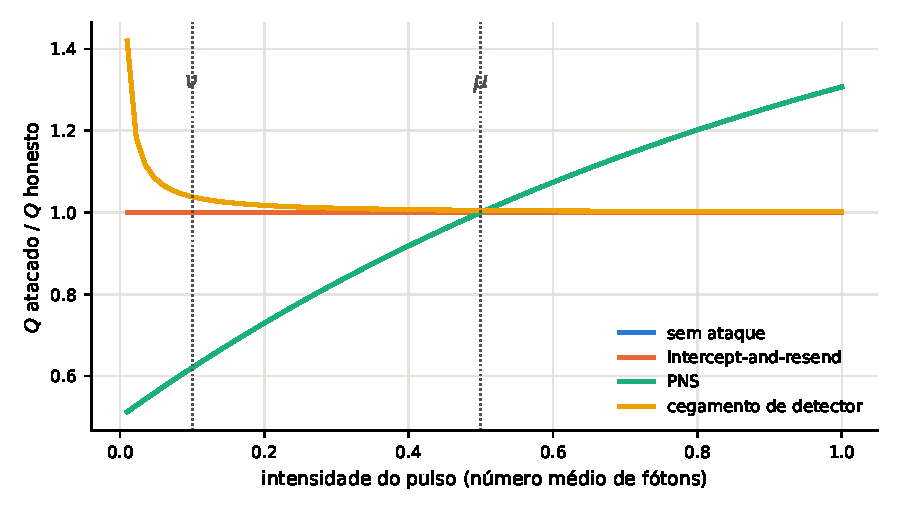
\includegraphics[width=0.86\textwidth]{figuras/assinaturas.pdf}
\caption{Ganho sob ataque dividido pelo ganho honesto, a 50~km, calculado
diretamente da física. O PNS mantém o ganho exatamente onde estava na intensidade
do sinal ($\mu$) e não consegue mantê-lo no \emph{decoy} fraco ($\nu$), onde quase
todo pulso é de fóton único; o intercept-and-resend não move o ganho em nenhuma
intensidade; o cegamento empurra o ganho acima do que a perda do canal permite.}
\label{fig:assinaturas}
\end{figure}

\subsection{Limites do receptor}

Três correções do próprio receptor entram no modelo, porque são o que impede que
aumentar a taxa de repetição seja gratuito. O tempo morto $\tau_d$ escala os
\emph{yields} por $1/(1 + r\tau_d)$, com $r$ a taxa bruta de cliques; o
\emph{afterpulsing} adiciona cliques descorrelacionados proporcionais à taxa de
cliques; e a dispersão cromática alarga o pulso, de modo que, no período de
\emph{slot} $T = 1/f$, a fração de fótons atribuída ao \emph{slot} vizinho produz
erro de intersímbolo $e_{\text{ISI}} = \tfrac12\,\mathrm{erfc}\!\left(T/2\sqrt{2}\sigma\right)$.
O teto do \emph{clock} pertence, portanto, ao vão e não ao receptor.

\section{Metodologia e Arquitetura de Simulação}

\subsection{Sessões, e não fórmulas}

A unidade de simulação é um episódio: um enlace operando por 10 minutos,
acertando contas a cada segundo --- $10^9$ pulsos por período a 1~GHz ---, com a
fibra derivando abaixo e um evento começando em um instante não anunciado. O
primeiro minuto é garantidamente livre de eventos e funciona como a calibração de
comissionamento que todo enlace implantado possui. A deriva de polarização usa o
modelo térmico mais vibração mais saltos discretos calibrado em
[Czegledi et al. 2016, Ramaswamy et al. 2026], e o resíduo que um compensador em
malha fechada não remove entra como desalinhamento óptico adicional. O
comprimento do vão é sorteado entre 20 e 70~km por episódio.

\subsection{Perfis adversos}

Todo ataque sorteia um perfil temporal --- degrau (40\%), rampa linear (35\%) ou
intermitente (25\%) --- e 40\% dos episódios de ataque carregam uma excursão
térmica simultânea. A severidade é escalada continuamente por um fator
$s(t) \in [0,1]$ que multiplica tudo o que o evento faz, de modo que um ataque em
rampa realmente intercepta uma fração crescente do tráfego. O contrato verificado
em teste é que $s=0$ é indistinguível de canal honesto.

\subsection{Atributos}

Dezessete atributos são calculados por período, todos relativos à linha de base do
próprio episódio. A escolha não é conveniência: um ganho absoluto é sobretudo uma
afirmação sobre o comprimento do vão, e as grandezas informativas são razões que
não deveriam ter mudado. Entram razões logarítmicas de ganho de sinal, de
\emph{decoy} e de vácuo; deslocamentos de taxa de erro; razões das cotas $Y_1^L$ e
$e_1^U$; ganho medido contra o previsto pela calibração; e três atributos de
janela móvel --- tendência do erro, volatilidade e a correlação entre o erro e
$|dT/dt|$. Esse último é o discriminador térmico: a taxa de deriva da
birrefringência é acoplada à \emph{variação} de temperatura, então uma excursão
térmica produz erro que sobe enquanto a temperatura se move e assenta quando ela
para --- correlação que o espião não possui. As colunas de verdade de referência
(desalinhamento real, transmitância real, $Y_1$ real) são explicitamente proibidas
no construtor de atributos.

\subsection{Protocolo de avaliação}

A separação treino/teste é \textbf{por episódio}, não por linha: linhas do mesmo
episódio compartilham calibração, comprimento de vão e realização de deriva.
Setenta por cento dos episódios vão para treino; destes, 20\% são reservados fora
do ajuste para calibrar o limiar de decisão. O divisor de feixe é gerado e
pontuado, mas não treinado: uma classe cujos atributos são idênticos aos de outra
ensina o modelo apenas a dividir ruído. As métricas reportadas são recall por
classe, alarmes falsos por hora de operação saudável (contando \emph{inícios} de
alarme) e precisão sob prior de 1\%; acurácia é deliberadamente omitida.

\section{Modelos de Inferência e Controle}

\subsection{Detectores}

Quatro famílias são comparadas sobre a mesma matriz de atributos: um limiar de
QBER calibrado por orçamento de alarme falso, que representa o que sistemas
implantados fazem hoje; \emph{random forest} [Breiman 2001]; máquina de vetores de
suporte com núcleo RBF [Cortes and Vapnik 1995]; e \emph{gradient boosting}
histogramático [Friedman 2001, Ke et al. 2017], implementados sobre
\emph{scikit-learn} [Pedregosa et al. 2011]. Duas camadas operacionais são
acrescentadas ao melhor modelo: um limiar de decisão sobre a massa de
probabilidade atribuída às classes de ataque, calibrado para um orçamento de
alarme falso em episódios não vistos, e uma histerese que exige persistência de
três períodos antes de contar um alarme.

\subsection{Agente de taxa de chave}

O ajuste do transmissor é formulado como processo de decisão sequencial
[Sutton and Barto 2018]. O estado é um vetor de dezesseis entradas contendo os
observáveis do período anterior relativos à calibração, a configuração corrente e
--- decisivo --- duas entradas \emph{absolutas} de regime de perda. As nove ações
são ajustes multiplicativos em $\mu$, $\nu$ e \emph{clock}, e aditivos na fração
de pulsos de sinal. A recompensa é a chave que se consegue \emph{provar} naquele
período, calculada pelas cotas de \emph{decoy} sobre contagens binomiais finitas,
e não a taxa assintótica. O treinamento usa ator-crítico com vantagem
generalizada [Mnih et al. 2016, Schulman et al. 2016] e otimizador Adam
[Kingma and Ba 2015], com redes implementadas em \emph{numpy}
[Harris et al. 2020] e retropropagação escrita manualmente, verificada contra
diferenças finitas.

\subsection{Sincronismo temporal}

O coeficiente termo-óptico da sílica implica aproximadamente 40~ps de atraso por
quilômetro por kelvin; em 50~km, um kelvin são dois nanossegundos, dez vezes a
janela típica de um detector com porta. O modelo compõe essa deriva com o
resíduo de um \emph{clock} recuperado do canal clássico. Quatro preditores são
comparados em laço fechado com latência: nenhuma correção, recalibração periódica
com tempo morto, filtro alfa-beta, e regressão \emph{ridge} sobre janela de
estimativas mais termômetro. A pontuação não é o RMS do desalinhamento, e sim a
eficiência de detecção e a taxa de chave que sobrevivem.

\subsection{Compensador temporal causal}

Para a compensação de polarização, compara-se a rede densa sobre janela achatada
com uma pilha de convoluções causais dilatadas [van den Oord et al. 2016,
Bai et al. 2018], alternativa às redes recorrentes [Hochreiter and Schmidhuber 1997]
com três vantagens específicas ao laço: a causalidade é estrutural e não
aprendida, o campo receptivo é um parâmetro de projeto, e a inferência é uma
multiplicação matricial em vez de um laço sobre o tempo.

\section{Avaliação Experimental: Detecção}

O conjunto compreende 168 episódios (24 por classe), 100.800 linhas e 90.720
períodos com atributos; 64.260 linhas de treino, das quais 44.280 para ajuste e
10.800 para calibração de limiar, e 22.680 períodos pontuados em teste.

\begin{table}[htbp]
\centering
\caption{Recall por classe em episódios retidos. O limiar de QBER responde apenas
``ataque'' ou ``normal'' e por isso zera a coluna de tipo.}
\label{tab:recall}
\footnotesize
\setlength{\tabcolsep}{4.5pt}
\begin{tabular}{@{}lccccc@{}}
\toprule
\textbf{Classe} & \textbf{Limiar} & \textbf{Random} & \textbf{SVM} & \textbf{Boos-} & \textbf{Boosting+} \\
 & \textbf{QBER} & \textbf{forest} & \textbf{(RBF)} & \textbf{ting} & \textbf{lim.+hist.} \\
\midrule
normal                & 0,993 & 0,948 & 0,924 & 0,938 & \textbf{0,968} \\
deriva térmica        & 0,000 & 0,864 & 0,651 & \textbf{0,875} & 0,863 \\
evento de perda       & 0,000 & \textbf{1,000} & 0,950 & \textbf{1,000} & 0,992 \\
intercept-and-resend  & 0,000 & \textbf{0,636} & 0,602 & 0,597 & 0,513 \\
PNS                   & 0,000 & \textbf{0,749} & 0,416 & 0,745 & 0,709 \\
cegamento de detector & 0,000 & 0,840 & 0,831 & \textbf{0,908} & 0,792 \\
\bottomrule
\end{tabular}
\end{table}

\begin{figure}[htbp]
\centering
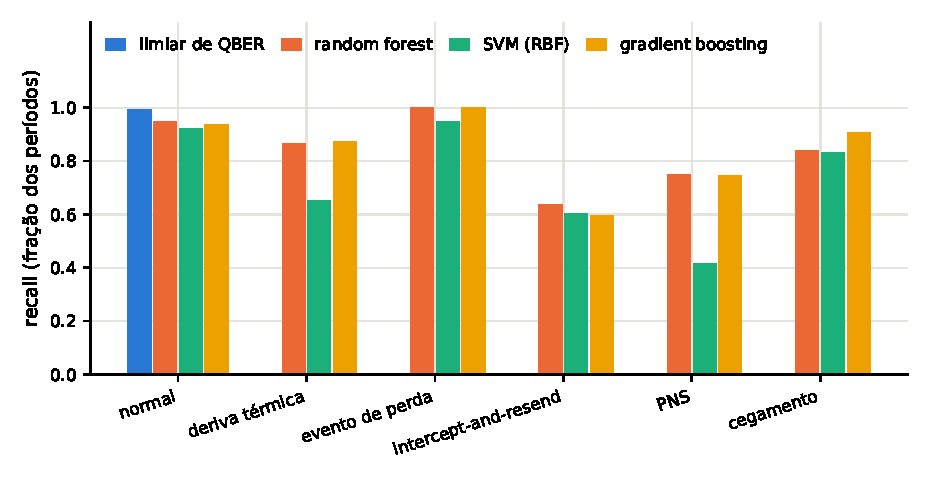
\includegraphics[width=0.92\textwidth]{figuras/recall.pdf}
\caption{Recall por classe. O limiar de QBER está calibrado para 1\% de alarme
falso no conjunto de treino --- é o que um operador faria com ele, e não um
espantalho.}
\label{fig:recall}
\end{figure}

O limiar de QBER, mesmo na versão binária, detecta 27\% dos períodos de
intercept-and-resend, 4\% dos de PNS, 11\% dos de cegamento e 3\% dos de evento de
perda. A assimetria é consequência da física: nenhum dos três últimos move a taxa
de erro. A Tabela~\ref{tab:operador} reporta as métricas que decidem
implantabilidade.

\begin{table}[htbp]
\centering
\caption{Métricas operacionais, período de acerto de 1~s. ``Alarmes/hora'' conta
inícios de alarme em períodos comprovadamente limpos.}
\label{tab:operador}
\small
\begin{tabular}{@{}lcccc@{}}
\toprule
\textbf{Detector} & \textbf{F1 macro} & \textbf{Alarme falso} & \textbf{Alarmes/hora} & \textbf{Precisão a 1\%} \\
\midrule
Limiar de QBER                     & 0,128 & 0,0073 & 1,6  & 0,103 \\
Random forest                      & \textbf{0,832} & 0,0525 & 8,9  & 0,155 \\
SVM (RBF)                          & 0,702 & 0,0761 & 36,4 & 0,113 \\
Gradient boosting                  & 0,830 & 0,0618 & 14,9 & 0,135 \\
Boosting + limiar de decisão       & 0,825 & 0,0373 & 11,0 & 0,200 \\
Boosting + limiar + histerese      & 0,818 & \textbf{0,0321} & \textbf{6,8} & \textbf{0,220} \\
\bottomrule
\end{tabular}
\end{table}

\subsection{Controle negativo}

O divisor de feixe não deixa assinatura alguma, e a resposta correta em seus
períodos é ``normal''. \emph{Random forest} e \emph{boosting} respondem isso em
91\% deles, e o SVM em 83\%: fronteiras suaves inventam ataque onde não há o que
ver. Uma taxa de detecção acima do acaso nessa classe indicaria vazamento do
gerador, e é por isso que ela é reportada separadamente e não incorporada à
acurácia.

\subsection{Qual física carrega a separação}

\begin{table}[htbp]
\centering
\caption{Ablações sobre a \emph{random forest}. Cada linha remove um bloco de
atributos.}
\label{tab:ablacoes}
\footnotesize
\setlength{\tabcolsep}{4.5pt}
\begin{tabular}{@{}lccccc@{}}
\toprule
\textbf{Variante} & \textbf{F1} & \textbf{Alarmes} & \textbf{PNS} & \textbf{Deriva} & \textbf{Interc.-} \\
 & \textbf{macro} & \textbf{/hora} & & \textbf{térmica} & \textbf{resend} \\
\midrule
Completa                      & \textbf{0,832} & 8,9   & 0,749 & 0,864 & 0,636 \\
Sem termômetro                & 0,768 & 80,7  & 0,753 & \textbf{0,425} & 0,536 \\
Sem observáveis de \emph{decoy} & 0,770 & 12,3  & \textbf{0,400} & 0,881 & 0,620 \\
Só QBER e ganho               & 0,622 & 104,3 & \textbf{0,098} & 0,390 & 0,542 \\
\bottomrule
\end{tabular}
\end{table}

A Tabela~\ref{tab:ablacoes} reproduz, como resultado de aprendizado, a afirmação
de segurança do protocolo: sem os observáveis de \emph{decoy}, o PNS deixa de ser
separável de forma confiável, e com apenas QBER e ganho torna-se praticamente
invisível. A remoção do termômetro derruba a deriva térmica pela metade e
multiplica os alarmes falsos por nove, porque deriva térmica e
intercept-and-resend produzem a mesma subida de QBER e se distinguem pela causa.

\subsection{Casos adversos}

\begin{table}[htbp]
\centering
\caption{Desempenho do \emph{gradient boosting} restrito aos períodos com ataque
em curso, por perfil temporal e por co-ocorrência térmica.}
\label{tab:adversos}
\small
\begin{tabular}{@{}lccc@{}}
\toprule
\textbf{Caso} & \textbf{Períodos} & \textbf{Recall} & \textbf{Detectado como algo} \\
\midrule
Degrau                           & 4.449 & 0,944 & 0,994 \\
Rampa                            & 2.678 & 0,778 & 0,970 \\
Intermitente                     & 1.811 & 0,562 & 0,834 \\
Com excursão térmica simultânea  & 2.685 & 0,631 & \textbf{1,000} \\
Sem excursão térmica             & 6.253 & 0,897 & 0,935 \\
\bottomrule
\end{tabular}
\end{table}

O ataque intermitente é o mais penalizado, por razão mecânica: metade dos
períodos rotulados como ataque são os intervalos entre rajadas, nos quais não há
nada a observar. A co-ocorrência térmica produz o achado mais informativo --- o
ataque é \emph{sempre} detectado como alguma coisa, mas o tipo correto cai de
0,897 para 0,631. A excursão térmica não esconde o ataque; ela rouba o rótulo.
Para comparação, o mesmo pipeline sobre um gerador restrito a ataques em degrau
isolados produz F1 macro de 0,93 e alarme falso de 1,4\%: \textbf{o número mais
alto mede um problema mais fácil}.

\subsection{A taxa de decisão, e não o modelo}

\begin{table}[htbp]
\centering
\caption{Mesmo pipeline com período de acerto de 5~s (12 episódios por classe).}
\label{tab:periodo}
\small
\begin{tabular}{@{}lcccc@{}}
\toprule
\textbf{Detector} & \textbf{F1 macro} & \textbf{Alarme falso} & \textbf{Alarmes/hora} & \textbf{Precisão a 1\%} \\
\midrule
Limiar de QBER                & 0,114 & 0,0181 & 0,5 & 0,012 \\
Random forest                 & \textbf{0,760} & 0,0798 & 5,0 & 0,103 \\
Gradient boosting             & 0,747 & 0,0843 & 3,9 & 0,101 \\
Boosting + limiar de decisão  & 0,718 & 0,0001 & 0,1 & 0,982 \\
Boosting + limiar + histerese & 0,694 & \textbf{0,0000} & \textbf{0,0} & \textbf{1,000} \\
\bottomrule
\end{tabular}
\end{table}

\begin{figure}[htbp]
\centering
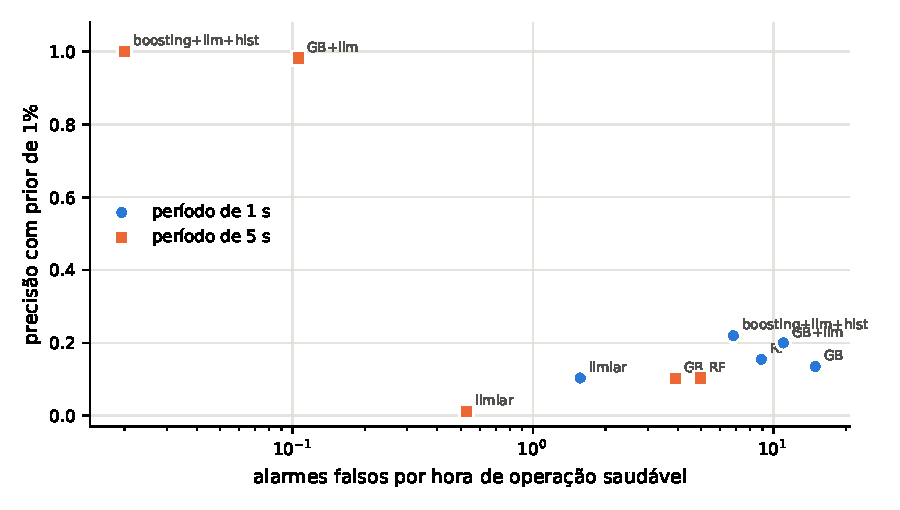
\includegraphics[width=0.90\textwidth]{figuras/ponto_operacao.pdf}
\caption{Alarmes falsos por hora contra precisão sob prior de 1\%, nos dois
períodos de acerto. O eixo horizontal é logarítmico. A mudança de regime não vem
de trocar o modelo, e sim de decidir cinco vezes menos e com cinco vezes mais
contagens por decisão.}
\label{fig:operacao}
\end{figure}

Com período de cinco segundos e limiar de decisão calibrado em episódios não
vistos, o alarme falso vai praticamente a zero e a precisão sob prior realista
passa de 0,22 para 1,00. O preço é atraso --- dezenas de segundos em vez de um ---
e o tipo do intercept-and-resend fraco, que passa a ser reportado como deriva
térmica ainda que o alarme suba. Trata-se de escolha de ponto de operação e não
de melhoria: um enlace que precise reagir em segundos permanece no período curto e
paga em chamados.

Registra-se uma armadilha metodológica encontrada nesse ponto. Calibrar o limiar
de decisão sobre as mesmas linhas usadas no ajuste produz limiar nulo --- o
\emph{boosting} praticamente não sinaliza períodos limpos que memorizou, embora
sinalize 6\% dos retidos --- e o alarme falso \emph{piora}. A calibração em 20\%
dos episódios de treino, fora do ajuste, é o que torna o mecanismo eficaz.

\section{Avaliação Experimental: Controle}

\subsection{Taxa de chave secreta}

O agente generalista foi treinado sorteando o vão entre 25 e 80~km por episódio. A
temperatura de amostragem foi escolhida em sementes de validação disjuntas do
teste, resultando em $T = 0{,}25$; o valor difere do encontrado na literatura de
políticas estocásticas porque, em vão longo, o ótimo é raso e a exploração custa
mais do que encontra.

\begin{table}[htbp]
\centering
\caption{Taxa de chave secreta provável, média de 24 episódios de teste por vão
(desvio-padrão entre episódios entre parênteses), em Mbit/s.}
\label{tab:chave}
\small
\begin{tabular}{@{}lcccc@{}}
\toprule
\textbf{Vão} & \textbf{Estático (comissionamento)} & \textbf{Agente} & \textbf{Oráculo} & \textbf{Ganho} \\
\midrule
25 km & 3,180 (0,451) & \textbf{3,782} (0,506) & 3,817 (0,584) & \textbf{+18,9\%} \\
35 km & 2,732 (0,425) & \textbf{3,092} (0,397) & 3,059 (0,417) & +13,2\% \\
50 km & 1,899 (0,319) & \textbf{2,128} (0,312) & 2,152 (0,353) & +12,1\% \\
65 km & 1,038 (0,169) & \textbf{1,138} (0,213) & 1,220 (0,244) & +9,6\% \\
80 km & 0,489 (0,072) & \textbf{0,532} (0,113) & 0,713 (0,107) & +8,8\% \\
\bottomrule
\end{tabular}
\end{table}

\begin{figure}[htbp]
\centering
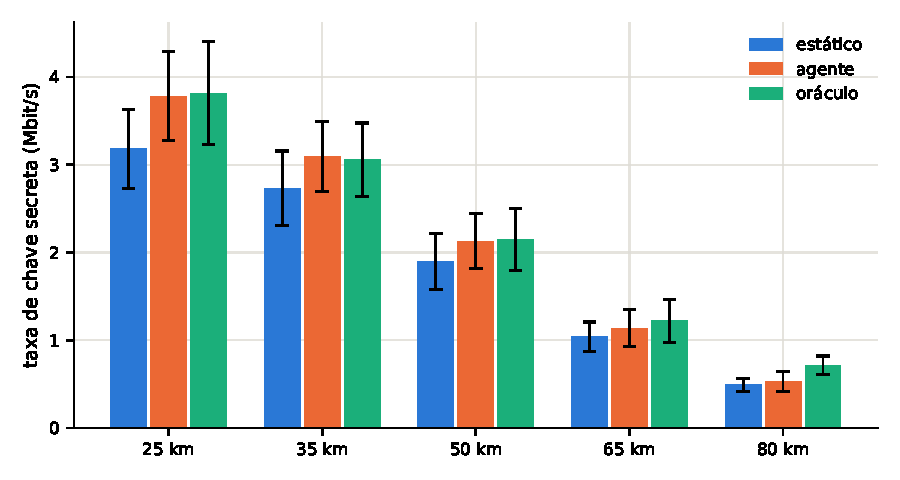
\includegraphics[width=0.88\textwidth]{figuras/taxa_chave.pdf}
\caption{Taxa de chave por vão. O oráculo lê o canal verdadeiro e reotimiza a cada
período; olha uma ação à frente e maximiza a taxa assintótica, sendo referência e
não teto --- em 35~km o agente o supera.}
\label{fig:chave}
\end{figure}

Até 50~km o agente recupera mais de 90\% da lacuna entre a linha de base e o
oráculo. Duas correções produziram esse resultado, e ambas merecem registro por
serem diagnósticos, não ajustes. A primeira: com atributos exclusivamente
relativos à calibração, o agente não distingue regimes --- uma queda de 20\% no
ganho é idêntica em 25 e em 80~km, embora os dois regimes exijam movimentos
opostos, pois em vão curto os detectores saturam e em vão longo a cota de fóton
único passa fome. Duas entradas absolutas levaram o vão de 80~km de $-14{,}7\%$ a
$+1{,}6\%$. A segunda: a varredura de temperatura de amostragem, que adicionou o
restante.

O comportamento aprendido é fisicamente interpretável. Em vãos curtos o agente
leva o \emph{decoy} ao piso da faixa ($\nu \approx 0{,}011$ contra os $0{,}1$ do
comissionamento), como a fórmula assintótica prescreve; em 80~km ele o eleva a
$\nu \approx 0{,}25$, que é exatamente onde a penalidade de estatística finita
passa a dominar --- e é também o único vão em que a margem sobre a linha de base
é a menor.

\subsection{Sincronismo temporal}

\begin{table}[htbp]
\centering
\caption{Taxa de chave a 50~km por sincronizador e largura de janela, em Mbit/s,
média de 12 execuções de uma hora.}
\label{tab:sinc}
\small
\begin{tabular}{@{}llcccc@{}}
\toprule
\textbf{Escuro} & \textbf{Janela} & \textbf{Sem correção} & \textbf{Recalib. 60~s} & \textbf{Filtro alfa-beta} & \textbf{Ridge + termômetro} \\
\midrule
$10$ Hz    & 200 ps  & 0,136 & 1,001 & 1,464 & \textbf{1,508} \\
           & 500 ps  & 0,309 & 1,631 & 1,958 & \textbf{1,971} \\
           & 1000 ps & 0,530 & 1,924 & \textbf{2,007} & \textbf{2,007} \\
$10^6$ Hz  & 200 ps  & 0,000 & 0,429 & 0,948 & \textbf{0,998} \\
           & 350 ps  & 0,000 & 0,536 & 1,064 & \textbf{1,099} \\
           & 1000 ps & 0,000 & 0,128 & 0,253 & 0,253 \\
\bottomrule
\end{tabular}
\end{table}

\begin{figure}[htbp]
\centering
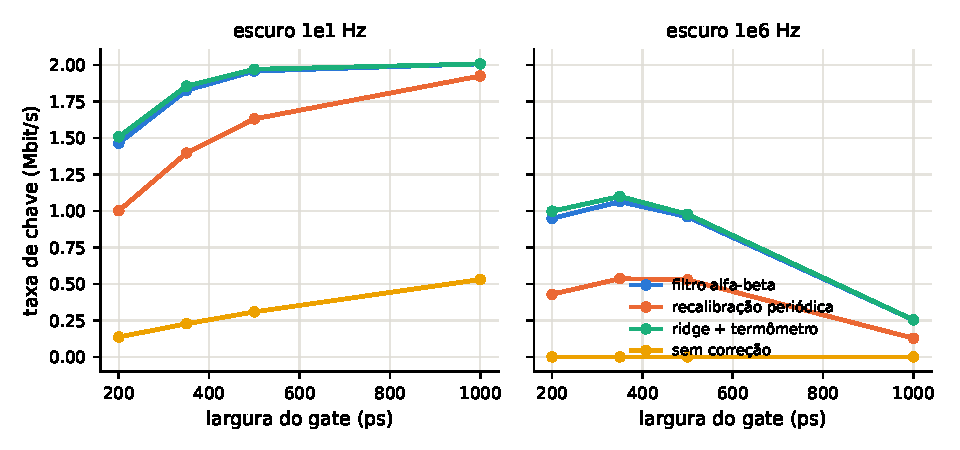
\includegraphics[width=0.95\textwidth]{figuras/sincronismo.pdf}
\caption{Taxa de chave contra largura da janela do detector, para dois regimes de
contagem de escuro. Com detector supercondutor silencioso, alargar a janela é
quase gratuito; com receptor ruidoso existe um ótimo interior, e sustentar uma
janela estreita exige rastreamento de qualidade.}
\label{fig:sinc}
\end{figure}

Três leituras importam mais que o ranqueamento. Primeira: um enlace calibrado e
deixado sem rastreamento perde 85\% da chave em uma hora com detector silencioso e
toda ela com detector ruidoso --- resultado que é o coeficiente termo-óptico da
sílica, não aprendizado de máquina. Segunda: recalibrar periodicamente custa nos
dois lados, pois a janela envelhece entre varreduras e a varredura interrompe o
enlace; a 60~s de intervalo entrega 83\% do rastreamento contínuo. Terceira: a
margem do preditor aprendido é modesta e aparece onde deveria --- janela estreita
e detector ruidoso ---, porque ele usa o termômetro e a componente térmica é
proporcional à \emph{variação} de temperatura, informação que um filtro
alfa-beta sobre a série do atraso não pode inferir.

\subsection{Compensador temporal causal}

\begin{table}[htbp]
\centering
\caption{Erro de validação por arquitetura, mesmas linhas e mesmo otimizador. O
campo receptivo é aritmética, não hiperparâmetro.}
\label{tab:tcn}
\small
\begin{tabular}{@{}lccc@{}}
\toprule
\textbf{Modelo} & \textbf{Campo receptivo} & \textbf{Parâmetros} & \textbf{MSE de validação} \\
\midrule
Rede densa (192, 192)             & 15 & 47.043 & \textbf{3.438} \\
TCN 32 canais, dilatações (1, 2)  & 7  & 5.923  & 7.035 \\
TCN 32 canais, dilatações (1,2,4) & 15 & 9.027  & 3.583 \\
TCN 48 canais, dilatações (1,2,4) & 15 & 17.923 & 3.586 \\
TCN 64 canais, dilatações (1,2,4) & 15 & 29.891 & 3.592 \\
\bottomrule
\end{tabular}
\end{table}

Com duas camadas dilatadas a pilha alcança sete atrasos; um período da banda de
vibração a 40~Hz corresponde a 12,5 passos de controle, de modo que sete atrasos
não cobrem uma oscilação inteira, e o erro dobra. Com três camadas o campo chega a
quinze, cobre o período, e o erro retorna ao patamar da rede densa. Capacidade
adicional não altera o resultado. Em laço fechado, a rede densa entrega 55.145
bit/s de chave finita, a regressão \emph{ridge} 54.722 e o TCN 54.636, contra
25.183 do filtro alfa-beta e 6.323 sem compensação. A conclusão honesta é que a
convolução causal \emph{iguala} a rede densa com um quinto dos parâmetros, e não a
supera: o viés indutivo de equivariância temporal economiza capacidade, não erro.

\section{Validação com Dados de Campo}
\label{sec:campo}

Todos os resultados anteriores foram medidos contra o simulador deste trabalho.
Esta seção confronta a física sobre a qual ele foi construído com dados de uma
rede implantada. [Dynes et al. 2019] depositaram sob licença CC-BY os dados das
figuras do artigo sobre a rede quântica metropolitana de Cambridge. Dois desses
arquivos são medições sobre as quais o modelo faz previsão: 575 instantâneos
diários, de novembro de 2016 a julho de 2018, da taxa de chave segura e do QBER
do enlace CAPE--TREL (10,6~km, 3,9~dB; BB84 com \emph{decoy states} a 1~GHz,
$\mu = 0{,}4$, $\nu = 0{,}1$, detectores de avalanche com eficiência de 30\% e
\emph{afterpulsing} de 3\%); e seis medidas do QBER contra a potência recebida de
um canal clássico de 100~Gbit/s multiplexado na mesma fibra.

O escopo do teste é determinado pelo conteúdo dos dados. Eles não trazem ganho
nem erro por intensidade, nem contagem de vácuo, nem ataque algum; o detector,
cuja metade dos atributos são observáveis de \emph{decoy}, não pode ser avaliado
sobre eles. O que se testa é a \emph{premissa} do detector e a \emph{física} que
o gerador, o agente e o sincronizador compartilham. A Figura~\ref{fig:campo}
resume os três testes.

\begin{figure}[htbp]
\centering
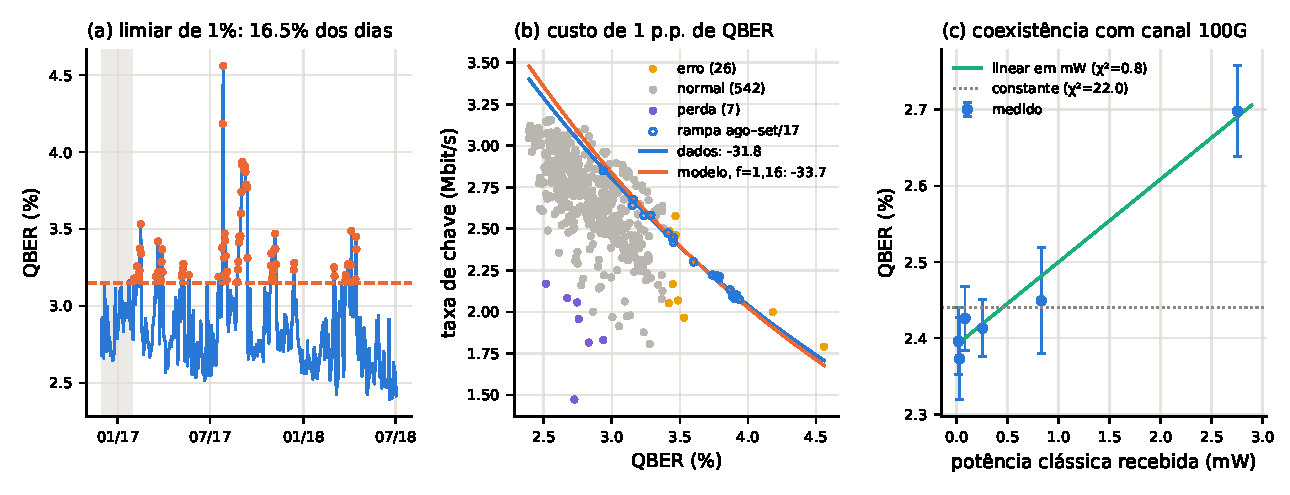
\includegraphics[width=\textwidth]{figuras/campo.pdf}
\caption{Dados do enlace CAPE--TREL da rede de Cambridge [Dynes et al. 2019].
(a)~QBER diário; em cinza, os 60 dias de comissionamento; linha tracejada, o
limiar calibrado para 1\% de alarme falso; pontos, os dias em que ele dispara.
(b)~Taxa de chave contra QBER; círculos, a excursão de agosto--setembro de 2017;
retas, a inclinação medida nela e a prevista pelo modelo; em cor, os dias
classificados como degradação por erro ou por perda. (c)~QBER contra a potência
clássica recebida, com o ajuste linear em miliwatts e a hipótese de QBER
constante.}
\label{fig:campo}
\end{figure}

\subsection{O limiar de QBER em dias benignos}

A regra implantada foi aplicada exatamente como no restante do trabalho: um
período de comissionamento define média e dispersão do QBER, e o limiar é posto no
quantil que dá o orçamento de alarme falso escolhido. Cada dia da série é benigno,
de modo que todo alarme é falso. A Tabela~\ref{tab:campo_limiar} mostra o
resultado.

\begin{table}[htbp]
\centering
\caption{Limiar de QBER calibrado no comissionamento, aplicado aos dias
seguintes da série de Cambridge. Todo alarme é falso.}
\label{tab:campo_limiar}
\footnotesize
\setlength{\tabcolsep}{4.5pt}
\begin{tabular}{@{}cccccc@{}}
\toprule
\textbf{Comissio-} & \textbf{Orça-} & \textbf{Limiar} & \textbf{Dias com} & \textbf{Episó-} & \textbf{Acima do} \\
\textbf{namento} & \textbf{mento} & & \textbf{alarme} & \textbf{dios} & \textbf{orçamento} \\
\midrule
30 dias & 1\% & 3,13\% & 16,5\% & 20 & 16,5$\times$ \\
60 dias & 1\% & 3,15\% & \textbf{16,5\%} & \textbf{17} & \textbf{16,5$\times$} \\
90 dias & 1\% & 3,39\% & 5,2\% & 7 & 5,2$\times$ \\
60 dias & 5\% & 3,12\% & 18,8\% & 20 & 3,8$\times$ \\
\bottomrule
\end{tabular}
\end{table}

Com 60 dias de comissionamento --- o mesmo número de períodos de linha de base
usado no simulador ---, o limiar dispara em um de cada seis dias, em 17 episódios
separados ao longo de 17 meses. É a premissa da Seção~\ref{sec:intro}, medida em enlace real: o
QBER de uma fibra implantada se move por conta própria, e um limiar sobre ele
gera alarmes pelo ambiente. Uma linha de base móvel de 30 dias reduz a taxa para
2,3\%, ainda o dobro do orçamento, e tem um defeito estrutural: aprende como
normal um ataque que entre em rampa, que é exatamente o perfil que o gerador
adverso inclui.

\subsection{O custo de um ponto de QBER}

A taxa de chave absoluta depende de parâmetros que [Dynes et al. 2019] não
publicam --- tempo morto, perda interna do receptor, tamanho do bloco finito ---,
e o modelo a superestima por um fator entre 1,4 e 2,4 conforme o tempo morto
assumido. A \emph{sensibilidade} $\mathrm{d}\ln R/\mathrm{d}E_\mu$, porém, é fixada
quase inteiramente pelos termos de entropia da cota GLLP
(Seção~\ref{sec:taxa}) e tem pouca liberdade: é a previsão adequada para o teste. A
Tabela~\ref{tab:campo_taxa} compara três estimativas nos dados com o modelo
avaliado no ponto de operação publicado, variando apenas o desalinhamento.

\begin{table}[htbp]
\centering
\caption{Sensibilidade da taxa de chave ao QBER, $\mathrm{d}\ln R/\mathrm{d}E_\mu$,
medida no enlace CAPE--TREL e prevista pelo modelo. O custo de um ponto
percentual é $1 - e^{s/100}$.}
\label{tab:campo_taxa}
\footnotesize
\begin{tabular}{@{}lcccc@{}}
\toprule
\textbf{Estimativa} & \textbf{Inclinação} & \textbf{IC 95\%} & \textbf{$R^2$} & \textbf{Custo de 1 p.p.} \\
\midrule
Série inteira & $-25{,}2$ & $\pm 2{,}2$ & 0,46 & 22\% \\
Intra-mês & $-31{,}2$ & $\pm 1{,}9$ & 0,66 & 27\% \\
Excursão ago--set/2017 & $\mathbf{-31{,}8}$ & $\pm \mathbf{1{,}1}$ & \textbf{0,994} & 27\% \\
\midrule
Modelo, $f = 1{,}16$ & $-33{,}7$ & --- & --- & 29\% \\
Modelo, $f = 1{,}10$ & $-31{,}1$ & --- & --- & 27\% \\
Modelo, $f = 1{,}00$ & $-27{,}4$ & --- & --- & 24\% \\
\bottomrule
\end{tabular}
\end{table}

A regressão sobre a série inteira é enviesada em direção a zero, e o viés tem
causa física: há dias em que a taxa cai sem que o QBER se mova --- perda, não
erro --- e variações lentas de perda ao longo do ano se sobrepõem à relação. Dois
estimadores removem o confundimento. O primeiro subtrai de ambas as grandezas a
média de cada mês. O segundo usa um experimento natural: entre 22 de agosto e 12
de setembro de 2017 o QBER subiu de 2,9\% para 3,9\% e foi corrigido em um único
dia, e ao longo dessa excursão a relação é exponencial com $R^2 = 0{,}994$. Os
dois concordam em $-31{,}5 \pm 1$.

O modelo, com a ineficiência de reconciliação $f = 1{,}16$ usada em todo o
trabalho, prevê $-33{,}7$: 6\% mais íngreme que a medida, cerca de duas vezes o
intervalo de confiança. A inclinação é sensível a um único parâmetro não
publicado, $f$, e com $f = 1{,}10$ o modelo reproduz a medida. A conclusão é que a
física de taxa de chave está correta e que o valor adotado para $f$ é
conservador para um sistema com reconciliação eficiente, na linha dos códigos
LDPC de taxa adaptativa que superam o Cascade [Elkouss et al. 2011].

Os dias ruins também se separam nos dois tipos de degradação que o gerador
produz. Tomando a inclinação medida como referência, 26 dias têm QBER mais de
dois desvios acima da mediana com a taxa sobre a reta --- degradação por
\emph{erro}, a classe de deriva térmica --- e 7 dias têm taxa até 47\% abaixo do
previsto com QBER normal --- degradação por \emph{perda}, a classe de evento de
perda. A distinção que o detector aprende entre essas duas classes existe numa
rede real.

\subsection{Coexistência com o canal clássico}

O ruído de espalhamento Raman gerado por um canal clássico na mesma fibra cresce
linearmente com a potência lançada [Eraerds et al. 2010, Kumar et al. 2015], e é
essa a forma do modelo de coexistência usado no trabalho. A
Tabela~\ref{tab:campo_coex} compara três formas funcionais sobre as seis medidas,
ponderadas pelas barras de erro publicadas.

\begin{table}[htbp]
\centering
\caption{Ajuste do QBER contra a potência clássica recebida (seis pontos).}
\label{tab:campo_coex}
\footnotesize
\begin{tabular}{@{}lccc@{}}
\toprule
\textbf{Forma} & $\boldsymbol{\chi^2}$ & \textbf{Graus de liberdade} & $\boldsymbol{p}$ \\
\midrule
QBER constante & 22,0 & 5 & 0,0005 \\
Linear em mW (Raman) & \textbf{0,80} & 4 & \textbf{0,94} \\
Linear em dBm & 8,4 & 4 & 0,08 \\
\bottomrule
\end{tabular}
\end{table}

A forma Raman é a que os dados sustentam, e o QBER constante é rejeitado. A
preferência, porém, depende quase inteiramente do ponto de maior potência
(+4,4~dBm): sem ele, a hipótese constante também se ajusta ($\chi^2 = 1{,}0$), e a
inclinação dos cinco pontos restantes ($0{,}065 \pm 0{,}092$~p.p./mW) é compatível
com a do ajuste completo ($0{,}109 \pm 0{,}024$~p.p./mW). Trata-se de consistência,
não de evidência independente.

A magnitude, por outro lado, não concorda. Com o coeficiente Raman, a largura de
filtro e a janela de detecção padrão do modelo, a subida prevista é de
6,1~p.p./mW, contra 0,11~p.p./mW medidos. Como o ruído Raman é proporcional ao
produto desses três parâmetros, apenas o produto é identificável; resolvendo o
modelo para reproduzir a medida, ele é 88 vezes menor que o padrão. Os limites de
potência clássica derivados com os valores padrão são, portanto, conservadores
por aproximadamente esse fator para um receptor da classe do de Cambridge.

\section{Discussão}

Três achados negativos foram preservados por serem informativos. O primeiro é o
divisor de feixe: uma classe que a física garante indetectável, e que serve de
detector de vazamento metodológico --- qualquer taxa de detecção acima do acaso
ali indica artefato. O segundo é o colapso do agente especialista: treinado
apenas em 50~km, recuperava toda a lacuna naquele vão e perdia 86\% em 80~km,
comportamento corrigido apenas com sorteio de vão em treino e com a observação do
regime absoluto. O terceiro é o próprio TCN, que não supera a arquitetura que
pretendia substituir.

Há também uma inversão de expectativa que vale registrar: a hipótese inicial de
que a recompensa por chave provável levaria o agente a \emph{elevar} a intensidade
do \emph{decoy}, por causa da estatística finita, é falsa no ponto de operação
estudado. Em bloco de um segundo a 1~GHz, mesmo $\nu = 0{,}01$ produz dezenas de
milhares de cliques de \emph{decoy} em vão metropolitano, e o agente reproduz a
prescrição assintótica. A penalidade de estatística finita só se manifesta em
80~km.

\section{Limitações e Validade Externa}

A limitação dominante é que os resultados de detecção e controle são \emph{in
silico}. As cotas e a taxa de chave são as publicadas [Ma et al. 2005, Gottesman
et al. 2004, Tomamichel et al. 2012], os ataques são escritos como modificação dos
\emph{yields}, e os parâmetros de deriva de polarização vêm de medições em fibra
implantada [Czegledi et al. 2016, Ramaswamy et al. 2026, Shi et al. 2026]. A
Seção~\ref{sec:campo} valida a premissa do detector e a física de taxa de chave e
de coexistência contra um enlace real, mas o detector em si não foi avaliado sobre
dado de campo, e um classificador treinado aqui é ponto de partida e não detector
pronto.

Essa validação tem limites próprios. Os dados publicados cobrem um único enlace,
em instantâneos diários, enquanto o simulador opera com período de um segundo:
testa-se a física e a premissa, não o detector na sua escala de tempo. Não há
temperatura nos dados, de modo que a atribuição das excursões de QBER ao ambiente
é inferida pela forma --- rampas lentas, correções abruptas --- e não medida; uma
série de temperatura de Cambridge no mesmo período permitiria testar o termômetro,
o atributo que carrega a separação entre deriva térmica e ataque. O limiar
comparado é a versão calibrada, a mais forte, e não o limiar fixo do fabricante:
nenhum dia da série passou de 4,6\% de QBER. E a concordância em taxa é de
sensibilidade, não de valor absoluto.

Há dado público para avançar além disso. [Tezzin et al. 2026] publicaram
medições de longo prazo de um sistema comercial operando entre o Instituto Militar
de Engenharia e o Centro Brasileiro de Pesquisas Físicas, no Rio de Janeiro, com
taxa de chave, QBER, visibilidade e temperaturas interna e externa registradas em
dois enlaces; o conjunto está depositado em repositório público
[Tezzin et al. 2026b]. Esse dado permite recalibrar o gerador --- e já contradiz
uma premissa deste trabalho, pois reporta QBER médio robusto ao \emph{nível} de
temperatura, com anomalias apenas durante gradientes acentuados, magnitude
inferior à adotada aqui. Confirma-se o mecanismo, corrige-se a escala. Por fim,
[Martin et al. 2024] disponibilizam, mediante solicitação, dados de rede
heterogênea em produção, que é o material adequado para testar transferência entre
fabricantes.

O que não existe publicamente é a outra metade: observáveis por intensidade
($Q_\nu$, $Y_0$, contagens de vácuo por bloco) exportados por equipamento
comercial, e enlaces sob ataque com rótulo. A literatura de \emph{quantum hacking}
publica demonstrações e figuras, não registros. Consequentemente, a validação
empírica das classes PNS e cegamento --- exatamente as que o limiar de QBER não
enxerga --- depende de experimento controlado em bancada, e não de dado
disponível.

Outras limitações: apenas um ataque por episódio; o estudo de taxa de decisão tem
dois pontos (1~s e 5~s); e em 80~km o agente ainda recupera apenas 19\% da lacuna
até o oráculo.

\section{Produto Tecnológico e Reprodutibilidade}

A implementação é um pacote Python que estende uma camada de física e dados para
redes quânticas construída sobre o simulador de eventos discretos SeQUeNCe
[Wu et al. 2021]. Os módulos novos são: a física de \emph{decoy states}; os
ataques como transformação de canal; o simulador de sessões; os detectores e seu
protocolo de avaliação; o ambiente e o agente de taxa de chave; o modelo de deriva
temporal com seus preditores; o compensador convolucional causal; e o módulo de
validação contra os dados de [Dynes et al. 2019]. Todas as redes
são implementadas em \emph{numpy} com retropropagação manual verificada contra
diferenças finitas. A suíte de testes conta 926 casos, entre os quais a verificação
de que força de ataque nula é indistinguível de canal honesto, de que o limiar de
decisão nulo reproduz exatamente a decisão \emph{argmax}, e de que a convolução
causal não enxerga o futuro. Os relatórios em HTML são gerados a partir dos mesmos
CSV que produzem as tabelas deste artigo.

\section{Conclusão}

Este trabalho mostra que a distinção entre espionagem e degradação ambiental em um
enlace de QKD com \emph{decoy states} é recuperável do registro público que as
duas pontas já trocam, acrescido de um termômetro. Sob avaliação adversa, um
classificador por \emph{gradient boosting} atinge F1 macro de 0,830 e detecta os
quatro ataques modelados, contra um dos quatro para o limiar de QBER calibrado ao
mesmo orçamento de alarme falso. As ablações localizam a separação: os
observáveis de \emph{decoy} carregam o PNS, o termômetro carrega a distinção entre
deriva térmica e intercept-and-resend. Sobre a mesma física, um agente
ator-crítico eleva a taxa de chave provável entre 8,8\% e 18,9\% sem tocar no
hardware, e um preditor com termômetro sustenta janelas de detecção estreitas
contra a deriva térmica do atraso.

O achado de maior consequência prática, porém, não é de modelagem: a precisão sob
prior realista é governada pela taxa de decisão do enlace. Reduzir a frequência de
decisão de um para cinco segundos, com limiar calibrado fora do ajuste, leva a
precisão de 0,22 a 1,00 --- um ganho que nenhuma troca de classificador produziu.

Os dados de campo da rede de Cambridge sustentam os fundamentos. Em 515 dias
benignos de um enlace implantado, o limiar de QBER calibrado para 1\% de alarme
falso disparou em 16,5\% dos dias; o custo medido de um ponto de QBER,
$-31{,}8 \pm 1{,}1$ em $\mathrm{d}\ln R/\mathrm{d}E_\mu$, concorda com o modelo
dentro de 6\%; e a penalidade de coexistência tem a forma Raman, com magnitude 88
vezes menor que a assumida por padrão. O passo seguinte é testar o termômetro
contra uma série de temperatura do mesmo enlace e produzir, em bancada, os
registros rotulados de ataque que a literatura ainda não publica.

\vspace{1.0em}

\begin{thebibliography}{99}
\small

\bibitem{} Bai, S., Kolter, J. Z., and Koltun, V. (2018). An empirical evaluation
of generic convolutional and recurrent networks for sequence modeling.
\textit{arXiv preprint} arXiv:1803.01271.

\bibitem{} Bennett, C. H. and Brassard, G. (1984). Quantum cryptography: public
key distribution and coin tossing. In \textit{Proceedings of the IEEE
International Conference on Computers, Systems and Signal Processing}, pages
175--179, Bangalore.

\bibitem{} Brassard, G., Lütkenhaus, N., Mor, T., and Sanders, B. C. (2000).
Limitations on practical quantum cryptography. \textit{Physical Review Letters},
85(6):1330--1333.

\bibitem{} Breiman, L. (2001). Random forests. \textit{Machine Learning},
45(1):5--32.

\bibitem{} Cortes, C. and Vapnik, V. (1995). Support-vector networks.
\textit{Machine Learning}, 20(3):273--297.

\bibitem{} Czegledi, C. B., Karlsson, M., Agrell, E., and Johannisson, P. (2016).
Polarization drift channel model for coherent fibre-optic systems.
\textit{Scientific Reports}, 6:21217.

\bibitem{} Diamanti, E., Lo, H.-K., Qi, B., and Yuan, Z. (2016). Practical
challenges in quantum key distribution. \textit{npj Quantum Information}, 2:16025.

\bibitem{} Dynes, J. F., Wonfor, A., Tam, W. W.-S., Sharpe, A. W., Takahashi, R.,
Lucamarini, M., Plews, A., Yuan, Z. L., et al. (2019). Cambridge quantum network.
\textit{npj Quantum Information}, 5:101. Dados sob CC-BY em
\url{https://doi.org/10.17863/CAM.44524}.

\bibitem{} Elkouss, D., Martinez-Mateo, J., and Martin, V. (2011). Information
reconciliation for quantum key distribution. \textit{Quantum Information and
Computation}, 11(3--4):226--238.

\bibitem{} Eraerds, P., Walenta, N., Legré, M., Gisin, N., and Zbinden, H. (2010).
Quantum key distribution and 1 Gbps data encryption over a single fibre.
\textit{New Journal of Physics}, 12(6):063027.

\bibitem{} Friedman, J. H. (2001). Greedy function approximation: a gradient
boosting machine. \textit{The Annals of Statistics}, 29(5):1189--1232.

\bibitem{} Gisin, N., Ribordy, G., Tittel, W., and Zbinden, H. (2002). Quantum
cryptography. \textit{Reviews of Modern Physics}, 74(1):145--195.

\bibitem{} Gottesman, D., Lo, H.-K., Lütkenhaus, N., and Preskill, J. (2004).
Security of quantum key distribution with imperfect devices. \textit{Quantum
Information and Computation}, 4(5):325--360.

\bibitem{} Harris, C. R., Millman, K. J., van der Walt, S. J., Gommers, R.,
Virtanen, P., Cournapeau, D., et al. (2020). Array programming with NumPy.
\textit{Nature}, 585:357--362.

\bibitem{} Hochreiter, S. and Schmidhuber, J. (1997). Long short-term memory.
\textit{Neural Computation}, 9(8):1735--1780.

\bibitem{} Hwang, W.-Y. (2003). Quantum key distribution with high loss: toward
global secure communication. \textit{Physical Review Letters}, 91(5):057901.

\bibitem{} Ke, G., Meng, Q., Finley, T., Wang, T., Chen, W., Ma, W., Ye, Q., and
Liu, T.-Y. (2017). LightGBM: a highly efficient gradient boosting decision tree.
In \textit{Advances in Neural Information Processing Systems}, pages 3146--3154.

\bibitem{} Kingma, D. P. and Ba, J. (2015). Adam: a method for stochastic
optimization. In \textit{International Conference on Learning Representations}.

\bibitem{} Kumar, R., Qin, H., and Alléaume, R. (2015). Coexistence of continuous
variable QKD with intense DWDM classical channels. \textit{New Journal of
Physics}, 17:043027.

\bibitem{} Lo, H.-K., Ma, X., and Chen, K. (2005). Decoy state quantum key
distribution. \textit{Physical Review Letters}, 94(23):230504.

\bibitem{} Lydersen, L., Wiechers, C., Wittmann, C., Elser, D., Skaar, J., and
Makarov, V. (2010). Hacking commercial quantum cryptography systems by tailored
bright illumination. \textit{Nature Photonics}, 4(10):686--689.

\bibitem{} Ma, X., Qi, B., Zhao, Y., and Lo, H.-K. (2005). Practical decoy state
for quantum key distribution. \textit{Physical Review A}, 72(1):012326.

\bibitem{} Mao, Y., Huang, W., Zhong, H., Wang, Y., Qin, H., Guo, Y., and Huang,
D. (2020). Detecting quantum attacks: a machine learning based defense strategy
for practical continuous-variable quantum key distribution. \textit{New Journal of
Physics}, 22. DOI: 10.1088/1367-2630/aba8d4.

\bibitem{} Martin, V., Brito, J. P., Ortíz, L., Méndez, R. B., Buruaga, J. S.,
Vicente, R. J., et al. (2024). MadQCI: a heterogeneous and scalable SDN-QKD
network deployed in production facilities. \textit{npj Quantum Information},
10:80.

\bibitem{} Mnih, V., Badia, A. P., Mirza, M., Graves, A., Lillicrap, T., Harley,
T., Silver, D., and Kavukcuoglu, K. (2016). Asynchronous methods for deep
reinforcement learning. In \textit{Proceedings of the 33rd International
Conference on Machine Learning}, pages 1928--1937.

\bibitem{} Pedregosa, F., Varoquaux, G., Gramfort, A., Michel, V., Thirion, B.,
Grisel, O., et al. (2011). Scikit-learn: machine learning in Python.
\textit{Journal of Machine Learning Research}, 12:2825--2830.

\bibitem{} Pirandola, S., Andersen, U. L., Banchi, L., Berta, M., Bunandar, D.,
Colbeck, R., et al. (2020). Advances in quantum cryptography. \textit{Advances in
Optics and Photonics}, 12(4):1012--1236.

\bibitem{} Ramaswamy, A., Rao, N. S. V., Chapman, J. C., and Alshowkan, M. (2026).
Analysis of polarization drift of optical signals over deployed aerial-inground
fiber connections. \textit{arXiv preprint} arXiv:2607.07629.

\bibitem{} Scarani, V., Bechmann-Pasquinucci, H., Cerf, N. J., Dušek, M.,
Lütkenhaus, N., and Peev, M. (2009). The security of practical quantum key
distribution. \textit{Reviews of Modern Physics}, 81(3):1301--1350.

\bibitem{} Schulman, J., Moritz, P., Levine, S., Jordan, M. I., and Abbeel, P.
(2016). High-dimensional continuous control using generalized advantage
estimation. In \textit{International Conference on Learning Representations}.

\bibitem{} Shi, S., Su, Y., Rahmouni, A., et al. (2026). Entanglement distribution
over a polarization-stabilized aerial fiber. \textit{arXiv preprint}
arXiv:2601.11753.

\bibitem{} Sutton, R. S. and Barto, A. G. (2018). \textit{Reinforcement learning:
an introduction}. MIT Press, 2nd edition.

\bibitem{} Tezzin, A., Uhdre, G. M., Martins, O., Rufo, S., and Carneiro, V. G. A.
(2026a). Long-term performance analysis of a commercial QKD device under
real-world deployment conditions. \textit{arXiv preprint} arXiv:2604.16236.

\bibitem{} Tezzin, A., Uhdre, G. M., Martins, O., Rufo, S., and Carneiro, V. G. A.
(2026b). Long-term performance dataset of a commercial QKD system operating under
tropical climate conditions in Rio de Janeiro, Brazil. \textit{IEEE DataPort}.
\url{https://ieee-dataport.org/documents/long-term-performance-dataset-commercial-qkd-system-operating-under-tropical-climate}.

\bibitem{} Tomamichel, M., Lim, C. C. W., Gisin, N., and Renner, R. (2012). Tight
finite-key analysis for quantum cryptography. \textit{Nature Communications},
3:634.

\bibitem{} van den Oord, A., Dieleman, S., Zen, H., Simonyan, K., Vinyals, O.,
Graves, A., Kalchbrenner, N., Senior, A., and Kavukcuoglu, K. (2016). WaveNet: a
generative model for raw audio. \textit{arXiv preprint} arXiv:1609.03499.

\bibitem{} Wang, W. and Lo, H.-K. (2019). Machine learning for optimal parameter
prediction in quantum key distribution. \textit{Physical Review A},
100(6):062334.

\bibitem{} Wu, X., Kolar, A., Chung, J., Jin, D., Zhong, T., Kettimuthu, R., and
Suchara, M. (2021). SeQUeNCe: a customizable discrete-event simulator of quantum
networks. \textit{Quantum Science and Technology}, 6(4):045027.

\bibitem{} Xu, F., Ma, X., Zhang, Q., Lo, H.-K., and Pan, J.-W. (2020). Secure
quantum key distribution with realistic devices. \textit{Reviews of Modern
Physics}, 92(2):025002.

\bibitem{} Xu, J., Ma, X., Liu, J., Zhang, C., Li, H., Zhou, X., and Wang, Q.
(2024). Automatically identifying imperfections and attacks in practical quantum
key distribution systems via machine learning. \textit{Science China Information
Sciences}, 67:202501.

\bibitem{} Zhao, Y., Fung, C.-H. F., Qi, B., Chen, C., and Lo, H.-K. (2008).
Quantum hacking: experimental demonstration of time-shift attack against
practical quantum-key-distribution systems. \textit{Physical Review A},
78(4):042333.

\end{thebibliography}

\end{document}
